\documentclass{article}
\usepackage[T2A]{fontenc} 
\usepackage[utf8]{inputenc} 
\usepackage[english,russian]{babel}
\usepackage{graphicx} 
\usepackage{amsmath}
\usepackage{amsfonts} 
\usepackage{titlesec}
\usepackage{listings}
\usepackage{float}
\usepackage{longtable}
\usepackage{titling} 
\usepackage{geometry} 
\usepackage{pgfplots}
\pgfplotsset{compat=1.9}
\usepackage{xcolor}
\definecolor{darkgreen}{RGB}{0,100,0}

\lstset{
  language=Python,
  basicstyle=\ttfamily,
  keywordstyle=\color{darkgreen},
  stringstyle=\color{purple},
  commentstyle=\color{green},
  morecomment=[l][\color{magenta}]{\#},
  frame=single, 
  showspaces=false, 
  showstringspaces=false, 
  numbers=left, 
  numberstyle=\tiny,
}

\titleformat{\section}
  {\normalfont\Large\bfseries}{\thesection}{1em}{}
\titleformat{\subsection}
  {\normalfont\large\bfseries}{\thesubsection}{1em}{}

\setlength{\droptitle}{-6em} 
\title{Контрольная работа по решению уравнений и систем уравнений}
\author{Винницкая Дина Сергеевна}
\date{Группа: Б9122-02-03-01сцт}

\geometry{a4paper, margin=2cm}

\begin{document}

\maketitle
\section*{Задание №1}

\begin{figure}[H]
    \centering
    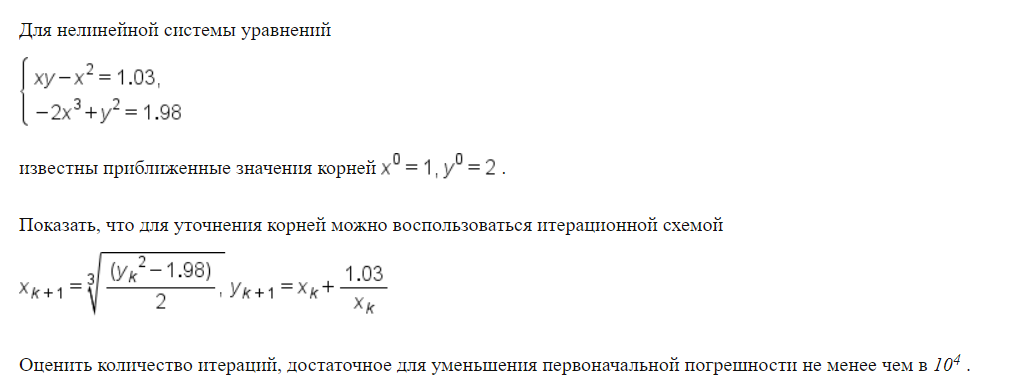
\includegraphics[width=1\textwidth]{last-kr.png}
    \label{fig:my_label}
\end{figure}
$$\textbf{Решение}$$
$\text{Первая итерация (\(k = 0\)):}$ \\
1. Вычисляем \(x_1\):
\[
x_1 = \sqrt[3]{\frac{(y_0^2 - 1.98)}{2}} = \sqrt[3]{\frac{(2^2 - 1.98)}{2}} = \sqrt[3]{\frac{4 - 1.98}{2}} = \sqrt[3]{\frac{2.02}{2}} = \sqrt[3]{1.01}
\]
$\text{Приблизительное значение:\( \quad x_1 \approx 1.0033\):}$\\
2. Вычисляем \(y_1\):
\[
y_1 = x_0 + \frac{1.03}{x_0} = 1 + \frac{1.03}{1} = 1 + 1.03 = 2.03
\]
$\text{Значения после первой итерации:\( \quad x_1 \approx 1.0033, \quad y_1 = 2.03\):}$\\
$\text{Вторая итерация (\(k = 1\)):}$\\
1. Вычисляем \(x_2\):
\[
x_2 = \sqrt[3]{\frac{(y_1^2 - 1.98)}{2}} = \sqrt[3]{\frac{(2.03^2 - 1.98)}{2}} = \sqrt[3]{\frac{4.1209 - 1.98}{2}} = \sqrt[3]{\frac{2.1409}{2}} = \sqrt[3]{1.07045}
\]
$\text{Приблизительное значение:\( \quad x_2 \approx 1.0225\):}$\\
2. Вычисляем \(y_2\):
\[
y_2 = x_1 + \frac{1.03}{x_1} = 1.0033 + \frac{1.03}{1.0033} \approx 1.0033 + 1.0267 = 2.03
\]
$\text{Значения после второй итерации:\( \quad x_2 \approx 1.0225, \quad y_2 \approx 2.03\):}$\\
$\text{Третья итерация (\(k = 2\)):}$\\
1. Вычисляем \(x_3\):
\[
x_3 = \sqrt[3]{\frac{(y_2^2 - 1.98)}{2}} = \sqrt[3]{\frac{(2.03^2 - 1.98)}{2}} = \sqrt[3]{\frac{4.1209 - 1.98}{2}} = \sqrt[3]{\frac{2.1409}{2}} = \sqrt[3]{1.07045}
\]
$\text{Приблизительное значение:\( \quad x_3 \approx 1.0228\):}$\\
2. Вычисляем \(y_3\):
\[
y_3 = x_2 + \frac{1.03}{x_2} = 1.0225 + \frac{1.03}{1.0225} \approx 1.0225 + 1.0077 = 2.0302
\]
$\text{Значения после третьей итерации:\( \quad x_3 \approx 1.0228, \quad y_3 \approx 2.0302\):}$\\
$\text{Итак, после трёх итераций значения \(x\) и \(y\) сходятся к:\( \quad x \approx 1.0228, \quad y \approx 2.0302\):}$\\
$\textbf{Количество итераций, необходимое для уменьшения ошибки не менее чем в \(10^4\), равно 3.}$

$$\textbf{Реализация алгоритма}$$
Для дополнительной проверки решения, реализуем алгоритм:
\begin{lstlisting}
def iterative_scheme(x0, y0, tolerance=1e-4):
    x = x0
    y = y0
    iteration = 0
    error = float('inf')
    
    while error > tolerance:
        x_new = ((y**2 - 1.98) / 2)**(1/3)
        y_new = x + 1.03 / x
        
        error = max(abs(x_new - x), abs(y_new - y))
        x, y = x_new, y_new
        iteration += 1
        
    return x, y, iteration
x0 = 1
y0 = 2

x_refined, y_refined, iterations = iterative_scheme(x0, y0)

x_refined, y_refined, iterations

\end{lstlisting}
Этот код инициализирует значения \(x\) и \(y\) заданными начальными приближениями и итеративно обновляет их с помощью предложенных формул. Процесс продолжается до тех пор, пока ошибка не станет меньше заданного порога.
Результат выполнения:
Уточненные значения корней: $x \approx 1.0229, \quad y \approx 2.0298$\\\\
Количество итераций, необходимое для уменьшения начальной ошибки не менее чем в \(10^4\), равно \(3\).\\\\
$\textbf{Таким образом в результате решения аналитическим путем и реализации программы можно}$
$\textbf{прийти к выводу о том, что необходимое количество итераций: 3}$\\\\
\textbf{Ответ: $\quad  \textbf{3 итерации}$}


\end{document}

